\documentclass[11pt,a4paper]{article}

%========================= FONTES E CODIFICACAO =========================
\usepackage[T1]{fontenc}
\usepackage[utf8]{inputenc}
\usepackage{mathptmx}
\usepackage[scaled=0.88]{helvet}
\usepackage{courier}
\usepackage{microtype}

% Sem padroes de hifenizacao em portugues nesta instalacao:
% penaliza hifenizacao para evitar quebras incorretas.
\hyphenpenalty=9000
\exhyphenpenalty=9000
\tolerance=2500
\emergencystretch=3em

%========================= GEOMETRIA =========================
\usepackage[a4paper,top=2.6cm,bottom=2.6cm,left=2.6cm,right=2.6cm,headheight=14pt]{geometry}

%========================= PACOTES =========================
\usepackage{xcolor}
\usepackage{graphicx}
\usepackage{booktabs}
\usepackage{tabularx}
\usepackage{longtable}
\usepackage{array}
\usepackage{enumitem}
\usepackage{titlesec}
\usepackage{fancyhdr}
\usepackage{caption}
\usepackage{float}
\usepackage{tcolorbox}
\tcbuselibrary{skins,breakable}
\usepackage{amsmath,amssymb}
\usepackage{listings}
\usepackage{xspace}
\usepackage{tikz}
\usetikzlibrary{arrows.meta,positioning,calc,fit,backgrounds}
\usepackage[hidelinks,pdfusetitle]{hyperref}

%========================= CORES =========================
\definecolor{lescblue}{HTML}{1F3A5F}
\definecolor{lescaccent}{HTML}{2E6DA4}
\definecolor{lescgray}{HTML}{4A4A4A}
\definecolor{lesclight}{HTML}{EEF3F8}
\definecolor{warncolor}{HTML}{8A3324}
\definecolor{warnlight}{HTML}{FBEEEA}
\definecolor{okcolor}{HTML}{2F5D3A}
\definecolor{oklight}{HTML}{EDF4EE}
\definecolor{rulegray}{HTML}{B8C4D0}
\definecolor{codebg}{HTML}{F6F8FA}
\definecolor{amber}{HTML}{8A6A14}
\definecolor{amberlight}{HTML}{FBF5E4}

%========================= SECOES =========================
\titleformat{\section}
  {\normalfont\Large\bfseries\color{lescblue}}
  {\thesection}{0.7em}{}[{\vspace{2pt}\color{rulegray}\titlerule[0.8pt]}]
\titleformat{\subsection}
  {\normalfont\large\bfseries\color{lescaccent}}
  {\thesubsection}{0.6em}{}
\titleformat{\subsubsection}
  {\normalfont\normalsize\bfseries\color{lescgray}}
  {\thesubsubsection}{0.5em}{}
\titlespacing*{\section}{0pt}{18pt}{9pt}
\titlespacing*{\subsection}{0pt}{13pt}{5pt}
\titlespacing*{\subsubsection}{0pt}{10pt}{4pt}

%========================= CABECALHO =========================
\pagestyle{fancy}
\fancyhf{}
\renewcommand{\headrulewidth}{0.4pt}
\renewcommand{\footrulewidth}{0pt}
\fancyhead[L]{\footnotesize\color{lescgray}Revisão técnica do port MAX 10}
\fancyhead[R]{\footnotesize\color{lescgray}LESC/UFC}
\fancyfoot[C]{\footnotesize\color{lescgray}\thepage}

%========================= LISTAS =========================
\setlist[itemize]{leftmargin=1.3em,itemsep=2pt,topsep=4pt,parsep=0pt}
\setlist[enumerate]{leftmargin=1.6em,itemsep=3pt,topsep=4pt,parsep=0pt}

%========================= CAIXAS =========================
\newcommand{\mkbox}[3]{%
\newtcolorbox{#1}[1][]{
  enhanced, breakable,
  colback=#3, colframe=#2,
  boxrule=0.4pt, left=8pt, right=8pt, top=7pt, bottom=7pt,
  arc=1.5pt,
  fonttitle=\bfseries\small\color{white},
  coltitle=white, colbacktitle=#2,
  attach boxed title to top left={xshift=6pt,yshift=-3pt},
  boxed title style={arc=1pt,boxrule=0pt},
  ##1}}
\mkbox{keybox}{lescaccent}{lesclight}
\mkbox{warnbox}{warncolor}{warnlight}
\mkbox{okbox}{okcolor}{oklight}
\mkbox{notebox}{amber}{amberlight}

% Ficha de cada problema
\newcommand{\campo}[1]{\vspace{5pt}\noindent{\bfseries\color{lescgray}#1}\par\vspace{1pt}}
\newcommand{\problema}[3]{%
  \vspace{8pt}
  \noindent\begin{tcolorbox}[enhanced,colback=lescblue,colframe=lescblue,
    boxrule=0pt,left=9pt,right=9pt,top=5pt,bottom=5pt,arc=2pt]
    {\color{white}\bfseries #1}\hfill{\color{white!80!lescblue}\small\bfseries #2}\\[1pt]
    {\color{white!82!lescblue}\small #3}
  \end{tcolorbox}\vspace{2pt}}

%========================= CODIGO =========================
\lstdefinestyle{rtl}{
  language=Verilog, basicstyle=\ttfamily\footnotesize, backgroundcolor=\color{codebg},
  frame=single, rulecolor=\color{rulegray}, framesep=4pt, xleftmargin=6pt, xrightmargin=6pt,
  keywordstyle=\color{lescblue}\bfseries, commentstyle=\color{okcolor}\itshape,
  stringstyle=\color{warncolor}, showstringspaces=false, columns=fullflexible,
  breaklines=true, morekeywords={logic,always_ff,always_comb,typedef,enum,localparam}}
\lstdefinestyle{sh}{
  language={}, basicstyle=\ttfamily\footnotesize, backgroundcolor=\color{codebg},
  frame=single, rulecolor=\color{rulegray}, framesep=4pt, xleftmargin=6pt, xrightmargin=6pt,
  commentstyle=\color{okcolor}\itshape, showstringspaces=false, columns=fullflexible, breaklines=true}
\lstset{style=rtl}

%========================= TABELAS =========================
\renewcommand{\arraystretch}{1.25}
\newcolumntype{L}[1]{>{\raggedright\arraybackslash}p{#1}}
\newcolumntype{C}[1]{>{\centering\arraybackslash}p{#1}}
\newcolumntype{Y}{>{\raggedright\arraybackslash}X}
\captionsetup[table]{font=small,labelfont={bf,color=lescblue},skip=5pt}
\captionsetup[figure]{font=small,labelfont={bf,color=lescblue}}
\renewcommand{\tablename}{Tabela}
\renewcommand{\figurename}{Figura}
\renewcommand{\contentsname}{Sumário}
\renewcommand{\lstlistingname}{Código}

\newcommand{\ps}{\ensuremath{\,\mathrm{ps}}\xspace}
\newcommand{\ns}{\ensuremath{\,\mathrm{ns}}\xspace}
\newcommand{\MHz}{\ensuremath{\,\mathrm{MHz}}\xspace}
\newcommand{\ms}{\ensuremath{\,\mathrm{ms}}\xspace}
\newcommand{\file}[1]{\texttt{\small #1}}

\begin{document}

%========================= CAPA =========================
\pagenumbering{alph}
\begin{titlepage}
\thispagestyle{empty}
\vspace*{1.2cm}
\noindent{\color{rulegray}\rule{\textwidth}{1.2pt}}
\vspace{0.9cm}

\noindent{\Huge\bfseries\color{lescblue}Revisão Técnica do Port do Sensor de \emph{Aging} para Intel MAX 10}

\vspace{0.7cm}
\noindent{\LARGE\color{lescaccent}Estado atual, correções, melhorias, plano de trabalho e critérios de aferição}

\vspace{0.5cm}
\noindent{\color{rulegray}\rule{\textwidth}{1.2pt}}
\vspace{1.2cm}

\noindent\begin{tcolorbox}[enhanced,colback=lesclight,colframe=lescaccent,boxrule=0.4pt,
  left=12pt,right=12pt,top=10pt,bottom=10pt,arc=2pt]
\small
\textbf{Objeto da revisão.} Os três commits da branch \texttt{max10-de10lite-port}
posteriores ao \emph{hand-off} do repositório: \texttt{a09d497} (07/10/2026),
\texttt{92c306b} (07/10/2026) e \texttt{b1f7635} (14/10/2026), todos restritos a
\texttt{max10\_port/}.

\vspace{5pt}
\textbf{Método.} Leitura integral do RTL, das restrições, da IP do PLL e dos relatórios
do Quartus; confronto com o plano (\file{docs/plano-port-max10.tex}) e com o RTL de
referência em Artix-7. Todas as afirmações quantitativas deste documento foram
\emph{medidas} --- por compilação no Quartus Prime Lite 25.1std (mesma versão usada na
implementação) e por simulação no Questa Starter 2025.2 com os modelos oficiais da Intel
(ALTPLL e átomos \texttt{fiftyfivenm}) --- e não estimadas.

\vspace{5pt}
\textbf{Público.} Equipe do port MAX~10 e coordenação. O texto pressupõe familiaridade
com a implementação Xilinx/Vivado e explica os equivalentes no Quartus à medida que
aparecem (resumo no Apêndice~\ref{ap:glossario}).
\end{tcolorbox}

\vfill
\noindent\begin{tabularx}{\textwidth}{@{}lX@{}}
\toprule
\textbf{Laboratório} & LESC --- Laboratório de Engenharia de Sistemas de Computação, UFC \\
\textbf{Data} & 29 de outubro de 2026 \\
\textbf{Base} & \texttt{max10-de10lite-port} @ \texttt{b1f7635} \\
\textbf{Ferramentas} & Quartus Prime Lite 25.1std.0 b1129; Questa Altera Starter 2025.2; Icarus Verilog \\
\textbf{Elaboração} & Revisão técnica conduzida com apoio de Claude Code (Anthropic) \\
\bottomrule
\end{tabularx}
\vspace{0.8cm}
\noindent{\color{rulegray}\rule{\textwidth}{0.8pt}}
\end{titlepage}

\pagenumbering{roman}
\setcounter{page}{1}
\tableofcontents
\clearpage
\pagenumbering{arabic}
\setcounter{page}{1}

%=========================================================================
\section*{Sumário executivo}
\addcontentsline{toc}{section}{Sumário executivo}
%=========================================================================

\begin{okbox}[title={Veredito}]
\textbf{A arquitetura do sensor de referência é implementável no MAX~10.} Os dois pilares
que motivavam dúvida estão demonstrados: (i) controle da lógica no nível da LUT,
com preservação contra otimização e fixação de posicionamento; (ii) três clocks alinhados
a partir de um mesmo VCO, com deslocamento dinâmico de fase de um deles --- o mecanismo
do auto-\emph{tuning}. Uma simulação de laço fechado do topo, com o modelo oficial do
PLL, calibra exatamente na contagem prevista pela análise de timing.
\end{okbox}

\begin{warnbox}[title={Mas o trabalho ainda está antes do Gate A}]
O que existe é uma \emph{prova de conceito de bancada}. Em relação ao objetivo da
branch, faltam ou estão errados: o laço não é contínuo (uma única medida por
\emph{reset}); a régua está em 178\ps quando o piso possível é 96\ps; a geometria
caminho/\emph{catcher} produz leitura \emph{silenciosamente} errada quando o caminho
fica rápido (defeito demonstrado em simulação); os testbenches não refletem o RTL;
o posicionamento do sensor não é reprodutível; e os binários versionados vêm de um
build quebrado. Nenhum desses pontos é um impedimento: todos têm correção conhecida
e verificável, descrita na Seção~\ref{sec:correcoes}.
\end{warnbox}

\begin{notebox}[title={O que permanece genuinamente incerto}]
O risco científico do projeto é quantitativo, não de viabilidade: o passo de fase do
MAX~10 é $\approx$4{,}9$\times$ mais grosso que o do Artix-7 e o nó de 55\,nm envelhece
mais devagar. Se o degrau de envelhecimento alcançável supera o ruído de medida só se
descobre em placa. A Seção~\ref{sec:tarefas} organiza o trabalho para chegar a esse número
o quanto antes.
\end{notebox}

\noindent\textbf{Como ler este documento.} A Seção~\ref{sec:contexto} resume o mecanismo do
sensor e os testes realizados. As Seções~\ref{sec:implementado} e~\ref{sec:contribuicao}
descrevem o que foi feito e o que isso já prova. A Seção~\ref{sec:correcoes} é o núcleo
prático: cada problema com evidência, causa, correção passo a passo e forma de verificação.
A Seção~\ref{sec:melhorias} trata de melhorias arquiteturais; a~\ref{sec:tarefas}, da
divisão do trabalho em paralelo; a~\ref{sec:afericao}, de como aferir que cada entrega
está correta.

%=========================================================================
\section{Contexto e método}
\label{sec:contexto}
%=========================================================================

\subsection{O mecanismo do sensor em uma página}

O sensor mede quanto \emph{tempo sobra} (o \emph{slack}) entre o instante em que um sinal
termina de atravessar um caminho lógico e o próximo flanco de clock. A Figura~\ref{fig:bloco}
mostra a estrutura implementada no MAX~10, que é a mesma da referência em Artix-7.

\begin{figure}[H]
\centering
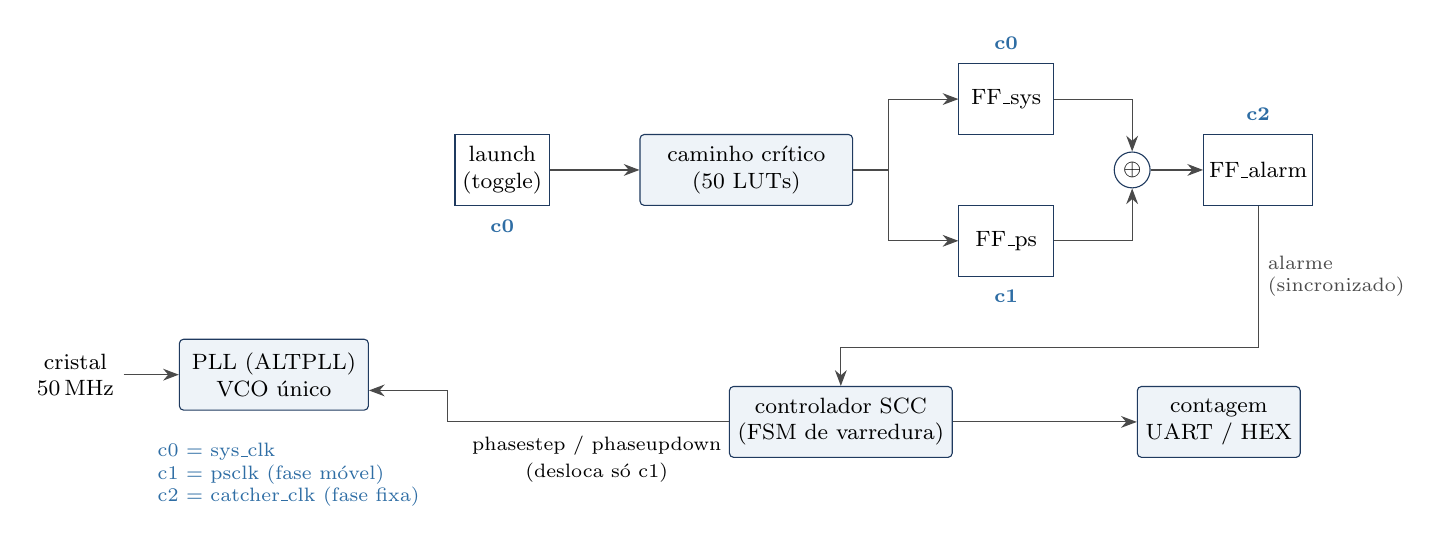
\begin{tikzpicture}[
  font=\footnotesize,
  blk/.style={draw=lescblue,fill=lesclight,rounded corners=1.5pt,minimum height=9mm,align=center,inner sep=3pt},
  ff/.style={draw=lescblue,fill=white,minimum width=12mm,minimum height=9mm,align=center,inner sep=2pt},
  arr/.style={-{Stealth[length=2mm]},lescgray},
  ck/.style={font=\scriptsize\bfseries,text=lescaccent}]
  % PLL e saidas
  \node[blk,minimum width=24mm] (pll) at (0,0) {PLL (ALTPLL)\\VCO único};
  \node[left=7mm of pll,align=center] (osc) {cristal\\50\,MHz};
  \draw[arr] (osc) -- (pll);
  \node[align=left,font=\scriptsize,text=lescaccent,anchor=north west] at (-1.6,-0.75)
    {c0 = sys\_clk\\c1 = psclk (fase móvel)\\c2 = catcher\_clk (fase fixa)};
  % caminho de dados
  \node[ff] (launch) at (2.9,2.6) {launch\\(toggle)};
  \node[blk,minimum width=27mm] (chain) at (6.0,2.6) {caminho crítico\\(50 LUTs)};
  \node[ff] (ffs) at (9.3,3.5) {FF\_sys};
  \node[ff] (ffp) at (9.3,1.7) {FF\_ps};
  \node[draw=lescblue,circle,inner sep=1.5pt] (xor) at (10.9,2.6) {$\oplus$};
  \node[ff] (ffa) at (12.5,2.6) {FF\_alarm};
  \draw[arr] (launch) -- (chain);
  \draw[arr] (chain.east) -- ++(0.45,0) |- (ffs.west);
  \draw[arr] (chain.east) -- ++(0.45,0) |- (ffp.west);
  \draw[arr] (ffs.east) -| (xor.north);
  \draw[arr] (ffp.east) -| (xor.south);
  \draw[arr] (xor) -- (ffa);
  % clocks de cada registrador
  \node[ck,below=0.5mm of launch] {c0};
  \node[ck,above=0.5mm of ffs] {c0};
  \node[ck,below=0.5mm of ffp] {c1};
  \node[ck,above=0.5mm of ffa] {c2};
  % controle
  \node[blk,minimum width=28mm] (scc) at (7.2,-0.6) {controlador SCC\\(FSM de varredura)};
  \node[blk] (out) at (12.0,-0.6) {contagem\\UART / HEX};
  \draw[arr] (ffa.south) -- node[right,font=\scriptsize,align=left] {alarme\\(sincronizado)} (12.5,0.35) -| (scc.north);
  \draw[arr] (scc) -- (out);
  \draw[arr] (scc.west) -- (2.2,-0.6) |- ($(pll.east)+(0,-0.2)$) node[pos=0.25,left,font=\scriptsize,align=right] {};
  \node[font=\scriptsize,anchor=north] at (4.1,-0.65) {phasestep / phaseupdown};
  \node[font=\scriptsize,anchor=north] at (4.1,-1.0) {(desloca só c1)};
\end{tikzpicture}
\caption{Estrutura do sensor. O PLL gera três clocks a partir do mesmo VCO; o controlador
move a fase do psclk até que as duas capturas do caminho divirjam.}
\label{fig:bloco}
\end{figure}

\begin{itemize}
  \item O registrador \texttt{launch} inverte a cada ciclo de \texttt{sys\_clk}, injetando
        uma transição no caminho a cada período $T$. A transição leva um tempo $d$ para
        atravessar o caminho.
  \item \texttt{FF\_sys} captura o fim do caminho no flanco de \texttt{sys\_clk}; \texttt{FF\_ps}
        captura o mesmo sinal no flanco de \texttt{psclk}, que o controlador \emph{adianta} em
        passos de tamanho $\Delta$ (o ``passo da régua'').
  \item Enquanto o flanco do psclk ocorre depois de o sinal estabilizar, as duas capturas
        coincidem e o XOR é 0. Quando o adiantamento $\delta = k\Delta$ ultrapassa o
        \emph{slack} $T-d$, \texttt{FF\_ps} passa a capturar o valor antigo, o XOR vai a 1
        e o \texttt{FF\_alarm} (no \texttt{catcher\_clk}) registra o alarme.
  \item O número de passos $k$ dado até o alarme é a medida:
        $\;k\,\Delta \approx T - d$. Envelhecimento aumenta $d$, logo $k$ diminui ao longo
        do tempo.
\end{itemize}

\begin{keybox}[title={Por que a régua é confiável}]
O passo $\Delta$ é uma fração fixa do período do VCO, que é travado no cristal da placa.
O caminho medido envelhece; a régua não. No Artix-7, $\Delta = T_\text{VCO}/56 \approx 19{,}8\ps$;
no MAX~10, $\Delta = T_\text{VCO}/8$, com piso de $\approx 96\ps$ (VCO a 1300\MHz).
\end{keybox}

\subsection{Testes realizados nesta revisão}

A Tabela~\ref{tab:testes} lista os experimentos que fundamentam as conclusões. Os arquivos
de cada um estão catalogados no Apêndice~\ref{ap:arquivos} e servem de ponto de partida para
a suíte de testes do repositório.

\begin{table}[H]
\centering
\caption{Experimentos executados (Quartus 25.1std Lite e Questa Starter 2025.2).}
\label{tab:testes}
\small
\begin{tabularx}{\textwidth}{@{}C{0.6cm} L{4.2cm} Y@{}}
\toprule
\textbf{\#} & \textbf{Experimento} & \textbf{Resultado} \\
\midrule
T1 & Compilação do projeto como está & Sucesso; 308 LEs; VCO 700\MHz; passo 178\ps; slack de c0 = 170{,}6\ns. Controlador presente (no build versionado ele havia sido otimizado para constante). \\
T2 & Simulação do ALTPLL (modelo Intel) com pulsos de \texttt{phasestep} & $-178{,}6\ps$ por passo em C1 com \texttt{phaseupdown=0}; seleção \texttt{011}=C1 e \texttt{100}=C2 confirmadas. \texttt{phasedone} fica baixo por \emph{meio} ciclo do scanclk. \\
T3 & PLL pedindo passos de 96, 100 e 120\ps & VCO 1300\MHz/96\ps (M=26); 1250\MHz/100\ps; 1050\MHz/119\ps. O piso é atingível. \\
T4 & \emph{Back-annotation} de posicionamento e dois builds limpos & 570 atribuições em nível de LC/FF; posicionamento idêntico entre builds. \\
T5 & Sensor travado $\times$ livre, alterando o RTL vizinho & Livre: atraso do caminho mudou 6{,}8\ns ($\approx$70 passos de 96\ps). Travado: posições idênticas; atraso de setup variou 21\ps, de hold 208\ps. \\
T6 & Fixar roteamento na edição Lite & Impossível: \emph{back-annotation} de roteamento não existe para MAX~10; partições incrementais são removidas pela licença Lite. \\
T7 & Somador 16 bits em cadeia de carry, sem trava, 3 variantes vizinhas & Atraso crítico 6{,}414 / 6{,}396 / 6{,}346\ns (dispersão de 68\ps). \\
T8 & Netlist para simulação com timing (SDF) & Não disponível para MAX~10 (``functional netlist is the only supported type''). \\
T9 & Laço fechado: topo + PLL oficial + cadeia como atraso do STA & Calibra em $\lfloor (T-d)/\Delta \rfloor + 1$ (primeiro passo além da borda) exatamente para $d$ = 29{,}2; 20; 12; 10{,}5\ns. \\
T10 & Idem, com caminho abaixo de 10\ns & Satura em 1065 passos independentemente de $d$ (defeito do \emph{catcher}, Seção~\ref{sec:catcher}). \\
T11 & Testbenches versionados & \file{max10\_aging\_top\_tb.sv} não compila; \file{scc\_controller\_tb.sv} falha em 3 testes e acusa 4 ``violações''. \\
\bottomrule
\end{tabularx}
\end{table}

%=========================================================================
\section{O que foi implementado}
\label{sec:implementado}
%=========================================================================

Os três commits criaram, praticamente do zero, o projeto Quartus em \file{max10\_port/hdl/}.
A Tabela~\ref{tab:modulos} descreve cada componente, sua correspondência com a referência
Vivado e sua situação.

\begin{table}[H]
\centering
\caption{Componentes implementados.}
\label{tab:modulos}
\small
\begin{tabularx}{\textwidth}{@{}L{3.3cm} Y L{2.6cm}@{}}
\toprule
\textbf{Componente} & \textbf{O que faz (e equivalente Vivado)} & \textbf{Situação} \\
\midrule
\file{aging\_pll.v} (IP ALTPLL) & 50\MHz $\rightarrow$ c0/c1/c2 a 5\MHz; c2 com +10\ns fixos; c1 com deslocamento dinâmico. Equivale ao \texttt{clk\_wiz\_0} (MMCM com PS dinâmico). & Funciona; VCO não está no máximo. \\
\file{critical\_path\_chain.sv} & 50 inversores instanciados como átomo \texttt{fiftyfivenm\_lcell\_comb} (\texttt{lut\_mask=16'h5555}, \texttt{dont\_touch}). Equivale a instanciar \texttt{LUT1}/\texttt{LUT3\_L} com \texttt{DONT\_TOUCH}. & Funciona: 50 LCs preservados. \\
\file{aging\_sensor\_core.sv} & FF\_sys, FF\_ps, XOR, FF\_alarm. Equivale ao \texttt{modern\_sensible}. & Correto; sem atributos de preservação. \\
\file{scc\_controller.sv} & FSM: espera \emph{lock}, sincroniza alarme, filtra, dá passos de fase por tempo, para no alarme. Equivale ao \texttt{controller\_controller}. & Funciona, mas é \emph{one-shot}. \\
\file{uart\_tx.sv}, \file{uart\_packet\_sender.sv} & Pacote de 5 bytes a cada 100\ms, 115200\,bps: \texttt{0xAA}, contagem, status, XOR. Equivale ao \texttt{sensor\_stream}. & Funciona; protocolo frágil. \\
\file{hex7seg.sv} + topo & Mostra a contagem em 4 displays; 7 LEDs de depuração. & Funciona. \\
\file{max10\_aging.sdc} & Clock de 50\MHz, \texttt{derive\_pll\_clocks}, \emph{false paths} do sensor. & Funciona; comentários desatualizados. \\
\file{max10\_aging\_top.qsf} & Pinos da DE10-Lite, 3 FFs fixados em LAB, SignalTap ligado. & Gerado pela GUI. \\
Testbenches (\file{src/sim/}) & Teste do controlador e de integração. & Desatualizados (T11). \\
Saídas de build & \file{db/}, \file{incremental\_db/}, \file{output\_files/} (\texttt{.sof}, \texttt{.pof}), bibliotecas de simulação. & Versionadas por engano; de um build quebrado. \\
\bottomrule
\end{tabularx}
\end{table}

\subsection{As duas correções posteriores estão certas}

\paragraph{\texttt{92c306b} --- seleção do contador e \emph{lock}.} No MAX~10,
\texttt{phasecounterselect} usa 000\,=\,todos, 001\,=\,M, 010\,=\,C0, 011\,=\,C1, 100\,=\,C2.
O valor anterior (\texttt{100}) deslocava o \emph{catcher}, não o psclk. O mesmo commit ligou
\texttt{pll\_locked} ao controlador; sem isso a porta fica em GND, o controlador permanece em
\emph{reset} e o Quartus o remove inteiro (``\emph{stuck at GND}'' em \file{map.rpt}). Ambas
confirmadas em T1 e T2.

\paragraph{\texttt{b1f7635} --- direção do deslocamento.} Com \texttt{phaseupdown=1} o psclk
\emph{atrasa}: o alarme só existiria se $\delta > d$, mas o \emph{catcher} amostra em +10\ns,
antes de o FF\_ps atualizar, e nunca o vê --- a fase ``passa direto''. Com \texttt{phaseupdown=0}
o psclk \emph{adianta} (como \texttt{psincdec=0} na referência) e mede-se $T-d$. Confirmado em T2 e T9.

\paragraph{O diagnóstico do \emph{handshake} também estava certo.} O comentário [C] do
controlador atribui o travamento ao pulso curto de \texttt{phasedone} e passa a sequenciar o
\emph{handshake} por tempo. T2 mostra que, no modelo da Intel, \texttt{phasedone} fica baixo
apenas entre o flanco de subida e o de descida do scanclk: uma FSM que só amostra em subida
nunca o observa. A solução por tempo é legítima; a melhoria possível (confirmar cada passo)
está na Seção~\ref{sec:melhorias}.

%=========================================================================
\section{Como isso contribui para o objetivo do projeto}
\label{sec:contribuicao}
%=========================================================================

O plano define quatro requisitos para o port. A Tabela~\ref{tab:requisitos} mostra o quanto
cada um avançou com a implementação atual somada aos testes desta revisão.

\begin{table}[H]
\centering
\caption{Progresso em relação aos requisitos do plano (Seção 1.1 do plano).}
\label{tab:requisitos}
\small
\begin{tabularx}{\textwidth}{@{}L{4.4cm} L{1.7cm} Y@{}}
\toprule
\textbf{Requisito} & \textbf{Estado} & \textbf{O que já está provado / o que falta} \\
\midrule
1. Medir o \emph{slack} com régua rastreável e caracterizada & Parcial & Provado: régua travada no cristal, passo em simulação e no fit. Falta: piso de 96\ps, medição do passo em placa, DNL. \\
2. Laço de auto-\emph{tuning} operacional & Parcial & Provado: varredura até o alarme, em laço fechado com o PLL oficial (T9). Falta: varredura contínua com retorno de fase, reaquisição, detecção de faixa. \\
3. Fidelidade em ps com incerteza declarada & Não iniciado & Depende de série temporal (req.~2) e de hardware. \\
4. Arquitetura independente de fabricante & Evidência favorável & Os mecanismos-chave portam (LUT, preservação, posicionamento, PLL dinâmico). A cadeia de inversores difere do \emph{dual-adder} RCA de referência; precisa de decisão documentada. \\
\bottomrule
\end{tabularx}
\end{table}

\begin{keybox}[title={O valor real do que foi feito}]
O maior risco técnico de qualquer port é descobrir tarde que a ferramenta não deixa
controlar a estrutura do circuito. Esse risco foi eliminado: a implementação atual
demonstra preservação de LUTs, PLL com deslocamento dinâmico e um laço que converge.
O que resta são problemas de engenharia com solução conhecida e a pergunta científica
de detectabilidade.
\end{keybox}

%=========================================================================
\section{O que precisa ser corrigido}
\label{sec:correcoes}
%=========================================================================

Cada item traz: o problema, a evidência, por que importa, como corrigir e como verificar a
correção. A ordem é a de prioridade; os itens C1--C4 bloqueiam o Gate A.

%-------------------------------------------------------------------------
\problema{C1. Repositório não reproduzível e binários de um build quebrado}{Crítico}
{Um clone limpo não compila, e o \texttt{.sof} versionado programa um sensor inoperante.}

\campo{Evidência}
\begin{itemize}
  \item \file{output\_files/*.sof/.pof} e \file{db/} datam de 06/10, antes da correção do
        \texttt{pll\_locked}; nesse build o controlador inteiro foi otimizado para constante.
  \item 194 arquivos e $\approx$15\,MB de saídas de ferramenta, arquivos \texttt{.bak},
        caminhos absolutos de Windows nos relatórios.
  \item O QSF ativa o SignalTap com \file{output\_files/stp1.stp}, que não está versionado, e
        aponta um testbench em \file{../../../../../../../Downloads/}.
  \item \file{src/constraints/max10\_aging.qsf} é um QSF órfão e divergente;
        \file{scripts/create\_project.tcl} continua um \emph{template}.
\end{itemize}

\campo{Por que importa}
Sem um build reproduzível a partir de texto versionado, ninguém consegue verificar o que outra
pessoa fez, e qualquer medida em placa fica sem rastreabilidade de qual circuito foi medido.

\campo{Como corrigir}
\begin{enumerate}
  \item Acrescentar ao \file{.gitignore} da raiz as regras do Quartus:
\begin{lstlisting}[style=sh]
# Quartus Prime (max10_port)
max10_port/hdl/db/
max10_port/hdl/incremental_db/
max10_port/hdl/output_files/
max10_port/hdl/greybox_tmp/
max10_port/hdl/simulation/
max10_port/hdl/build/
max10_port/hdl/*.qws
max10_port/hdl/*.rpt
*.bak
*.bak[0-9]
\end{lstlisting}
  \item Remover do índice (sem apagar a cópia local de quem estiver trabalhando):
\begin{lstlisting}[style=sh]
git rm -r --cached max10_port/hdl/db max10_port/hdl/incremental_db \
  max10_port/hdl/output_files max10_port/hdl/simulation max10_port/hdl/greybox_tmp
git rm --cached max10_port/hdl/*.bak max10_port/hdl/src/**/*.bak max10_port/hdl/*.qws
\end{lstlisting}
  \item Manter versionados apenas: RTL, SDC, a IP (\file{aging\_pll.v}, \file{.qip}, \file{.ppf})
        e \emph{um} QSF. Recomenda-se que o QSF passe a ser gerado por
        \file{scripts/create\_project.tcl} (preenchendo os TODOs com as listas de arquivos e
        atribuições), como nos projetos Vivado; o QSF da GUI vira saída.
  \item Desligar o SignalTap no QSF de referência (\texttt{ENABLE\_SIGNALTAP OFF}); quem precisar
        dele liga localmente.
  \item Trazer o testbench de gate-level para \file{src/sim/} e corrigir o caminho, ou remover
        as linhas \texttt{EDA\_TEST\_BENCH\_*}.
  \item Para distribuir bitstreams, seguir a convenção do Nexys: uma pasta
        \file{hdl/bitstreams/} com o \texttt{.sof} \emph{e} o hash do commit de origem no nome.
  \item Fixar a versão: registrar em \file{hdl/README.md} ``Quartus Prime Lite 25.1std.0
        Build 1129'' e exigir essa versão de toda a equipe.
\end{enumerate}

\campo{Como verificar}
Em um clone limpo: \texttt{scripts/check\_layout.sh}, depois \texttt{scripts/create\_project.sh}
e \texttt{scripts/build\_bitstream.sh} terminam sem erro; o \file{map.rpt} não contém
``\emph{stuck at GND}'' para registradores do \texttt{scc\_controller}; \texttt{git status}
fica limpo após o build.

%-------------------------------------------------------------------------
\problema{C2. O laço de auto-tuning não é contínuo}{Crítico}
{Uma medida por \emph{reset} manual: impossível obter série temporal, $\sigma_\text{resid}$ ou rastrear deriva.}

\campo{Evidência}
No controlador atual, o estado \texttt{S\_DONE} é terminal (linhas 249--251 de
\file{scc\_controller.sv}). A referência, \file{controller\_controller.sv}, trava o valor,
devolve a fase a zero e recomeça sozinha.

\campo{Por que importa}
É o requisito~2 do plano e o critério do Gate A (``laço rastreando uma borda deslocada'').
Toda a análise estatística depende de muitas medidas sucessivas.

\campo{Como corrigir}
Acrescentar à FSM os estados de retorno de fase da referência, preservando o
\emph{handshake} temporizado que já funciona (Figura~\ref{fig:fsm}).

\begin{figure}[H]
\centering
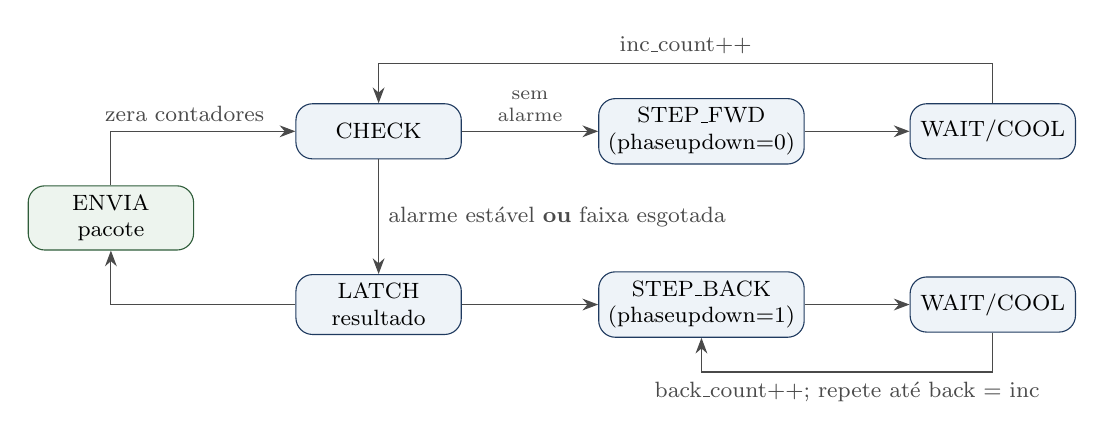
\begin{tikzpicture}[font=\footnotesize,
  st/.style={draw=lescblue,fill=lesclight,rounded corners=6pt,minimum width=21mm,minimum height=7mm,align=center},
  arr/.style={-{Stealth[length=2mm]},lescgray}]
  \node[st] (chk) at (0,0) {CHECK};
  \node[st] (fwd) at (4.1,0) {STEP\_FWD\\(phaseupdown=0)};
  \node[st] (wf) at (7.8,0) {WAIT/COOL};
  \node[st] (lat) at (0,-2.2) {LATCH\\resultado};
  \node[st] (bck) at (4.1,-2.2) {STEP\_BACK\\(phaseupdown=1)};
  \node[st] (wb) at (7.8,-2.2) {WAIT/COOL};
  \node[st,fill=oklight,draw=okcolor] (snd) at (-3.4,-1.1) {ENVIA\\pacote};
  \draw[arr] (chk) -- node[above,font=\scriptsize,align=center]{sem\\alarme} (fwd);
  \draw[arr] (fwd) -- (wf);
  \draw[arr] (wf.north) -- ++(0,0.5) -| node[pos=0.25,above]{inc\_count++} (chk.north);
  \draw[arr] (chk) -- node[right]{alarme estável \textbf{ou} faixa esgotada} (lat);
  \draw[arr] (lat) -- (bck);
  \draw[arr] (bck) -- (wb);
  \draw[arr] (wb.south) -- ++(0,-0.5) -| node[pos=0.25,below]{back\_count++; repete até back = inc} (bck.south);
  \draw[arr] (lat.west) -| (snd.south);
  \draw[arr] (snd.north) |- node[pos=0.7,above]{zera contadores} (chk.west);
\end{tikzpicture}
\caption{FSM contínua proposta. O retorno é feito pelo mesmo número de passos dados para frente,
de modo que cada varredura começa sempre da fase zero.}
\label{fig:fsm}
\end{figure}

\noindent Esboço dos pontos novos (a lógica de \emph{timer} do \emph{handshake} é a atual,
reaproveitada nos dois sentidos):
\begin{lstlisting}
// phaseupdown passa a ser controlado pela FSM: 0 = adianta (medicao), 1 = atrasa (retorno)
assign phaseupdown = (dir == DIR_BACK);

S_CHECK: if (alarm_stable || inc_count == MAX_STEPS) next_state = S_LATCH;
         else                                         next_state = S_STEP_FWD;
S_LATCH: next_state = (inc_count == 0) ? S_RESTART : S_STEP_BACK;
// S_STEP_BACK/S_WAIT_BACK: mesmo handshake temporizado; back_count++ ao fim de cada passo
S_WAIT_BACK_DONE: next_state = (back_count == inc_count) ? S_RESTART : S_STEP_BACK;
S_RESTART: begin inc_count <= 0; back_count <= 0; seq <= seq + 1; next_state = S_CHECK; end

// no S_LATCH: result <= inc_count; result_valid <= 1;
//             out_of_range <= (inc_count == MAX_STEPS);  // borda nao encontrada
\end{lstlisting}
Pontos de atenção:
\begin{itemize}
  \item \texttt{MAX\_STEPS} deve ser um parâmetro de topo derivado de $T$ e $\Delta$
        (uma volta completa: $T/\Delta$); se atingido, a medida é marcada inválida, nunca reportada como número.
  \item O resultado é \emph{registrado} em \texttt{S\_LATCH} e permanece estável durante o
        retorno; o pacote UART lê sempre o último resultado válido, com número de sequência.
  \item Após o retorno, aguardar alguns ciclos de \texttt{catcher\_clk} antes do próximo
        \texttt{CHECK} para o alarme da varredura anterior se dissipar (zerar o filtro).
\end{itemize}

\campo{Como verificar}
Testbench com o modelo oficial do PLL e cadeia comportamental (base pronta, T9): (a) em
$d$ fixo, 20 varreduras consecutivas devolvem a mesma contagem; (b) mudando $d$ durante a
simulação (degrau de $+500\ps$), a contagem seguinte cai de $\lceil 500/\Delta\rceil$ ou
$\lfloor 500/\Delta\rfloor$ passos; (c) após cada retorno, a fase medida de c1 em relação a c0
volta a 0\ps; (d) com caminho impossível (sem alarme), a FSM marca \texttt{out\_of\_range} e
recomeça, sem travar.

%-------------------------------------------------------------------------
\problema{C3. Geometria caminho/catcher: leitura errada sem aviso}{Crítico}
{Se o caminho ficar mais rápido que o atraso do \emph{catcher}, o sensor passa a medir o \emph{catcher}.}
\label{sec:catcher}

\campo{Evidência}
T10: com a cadeia abaixo de $\approx$10\ns, a contagem satura em 1065 passos
($1065 \times 178{,}6\ps \approx 190\ns = T - 10\ns$), qualquer que seja o atraso real. O corner
rápido do STA dá $d \approx 10{,}5\ns$: margem de apenas $\approx$0{,}5\ns.

\campo{Por que acontece}
A Figura~\ref{fig:janela} mostra a janela de tempo. O XOR só reflete a comparação correta
entre o flanco de \texttt{sys\_clk} (quando FF\_sys atualiza) e o próximo flanco de psclk
(quando FF\_ps atualiza de novo). O \emph{catcher}, em $+c$ após \texttt{sys\_clk}, precisa cair
dentro dessa janela:
\[
  t_{co} + t_{xor} \;<\; c \;<\; T - \delta .
\]
No limiar de alarme, $\delta = T - d$, então a condição vira $c < d$. Se $c > d$, o psclk
adiantado ``passa'' por cima do \emph{catcher} antes de o caminho falhar, e o alarme dispara em
$\delta = T - c$: a leitura vira $\min(T-d,\;T-c)$.

\begin{figure}[H]
\centering
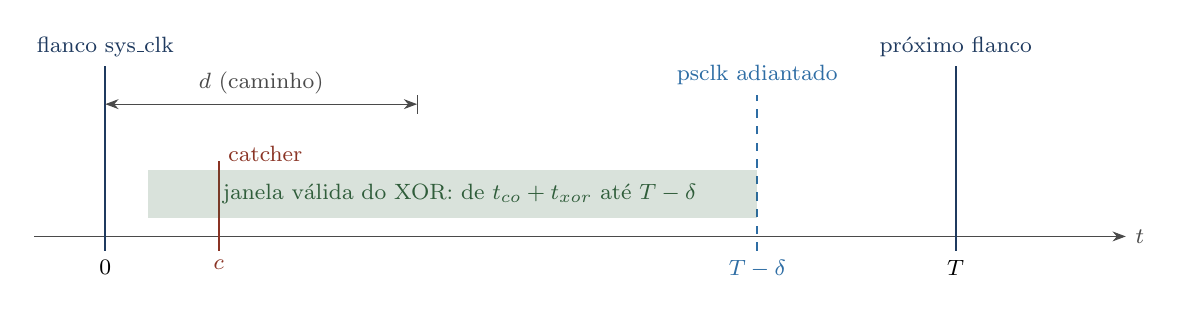
\begin{tikzpicture}[font=\footnotesize,x=0.9cm,y=0.6cm]
  \draw[lescgray,-{Stealth}] (0,0) -- (15.4,0) node[right] {$t$};
  \foreach \x/\l in {1/{$0$},13/{$T$}} { \draw[lescblue,thick] (\x,-0.3) -- (\x,3.6); \node[below] at (\x,-0.3) {\l}; }
  \node[lescblue,above] at (1,3.6) {flanco sys\_clk};
  \node[lescblue,above] at (13,3.6) {próximo flanco};
  \draw[lescaccent,thick,dashed] (10.2,-0.3) -- (10.2,3.0); \node[lescaccent,below] at (10.2,-0.3) {$T-\delta$};
  \node[lescaccent,above] at (10.2,3.0) {psclk adiantado};
  \draw[warncolor,thick] (2.6,-0.3) -- (2.6,1.6); \node[warncolor,below] at (2.6,-0.3) {$c$};
  \node[warncolor,right] at (2.6,1.75) {catcher};
  \fill[okcolor,opacity=0.18] (1.6,0.4) rectangle (10.2,1.4);
  \node[okcolor] at (6.0,0.9) {janela válida do XOR: de $t_{co}+t_{xor}$ até $T-\delta$};
  \draw[lescgray,{Stealth}-{Stealth}] (1,2.8) -- node[above]{$d$ (caminho)} (5.4,2.8);
  \draw[lescgray] (5.4,2.6) -- (5.4,3.0);
\end{tikzpicture}
\caption{Janela de amostragem. A medida só é válida enquanto o \emph{catcher} ($c$) estiver
antes de $T-\delta$. Como o alarme legítimo ocorre em $\delta = T-d$, é preciso $c < d$ com folga
em todos os corners.}
\label{fig:janela}
\end{figure}

\campo{Como corrigir}
\begin{enumerate}
  \item \textbf{Regra de projeto}, a ser cumprida em todos os corners de PVT e ao longo do
        envelhecimento:
        \[
          t_{co} + t_{xor} + \text{margem} \;<\; c \;<\; d_\text{min} - \text{margem},
          \qquad d_\text{max,envelhecido} < T - \text{margem}.
        \]
  \item \textbf{Reduzir $c$}: hoje são 10\ns; bastam $\approx$2--3\ns (o suficiente para
        FF\_sys atualizar e o XOR assentar). Alterar \texttt{clk2\_phase\_shift} na IP.
  \item \textbf{Garantir por STA o lado inferior}: substituir os dois \texttt{set\_false\_path}
        de clk[0]/clk[1] para clk[2] por uma restrição que obrigue o XOR a assentar antes do
        \emph{catcher}, por exemplo
\begin{lstlisting}[style=sh]
# o XOR precisa estar estavel antes do catcher (c), com folga
set_max_delay -from [get_registers {*ff_sys_clk_q *ff_psclk_q}] \
              -to   [get_registers {*ff_alarm_q}] 1.500
\end{lstlisting}
        e conferir no relatório que o caminho fecha.
  \item \textbf{Dimensionar o caminho} (ver também Seção~\ref{sec:melhorias}): com
        $T = 200\ns$ e $d \approx 29\ns$, só 15\% do período é caminho, o que aproxima $d_\text{min}$
        de $c$ e desperdiça sinal de envelhecimento (que é proporcional a $d$). Escolher $T$ e o
        comprimento do caminho juntos, pela regra acima.
  \item \textbf{Detector de saturação} no RTL: se o resultado ficar a menos de alguns passos de
        $(T-c)/\Delta$, marcar a medida como inválida no pacote. Isso transforma um erro
        silencioso em um erro visível.
  \item \textbf{Modo de diagnóstico em placa}: o \texttt{phasecounterselect} também alcança
        C2, então o \emph{catcher} pode ser varrido dinamicamente para localizar, no silício, a
        fronteira de saturação.
\end{enumerate}

\campo{Como verificar}
Repetir T9/T10 com os novos parâmetros: para $d$ variando do corner rápido ao lento
(acrescido de, por exemplo, 10\% de envelhecimento), a contagem deve seguir
$\lfloor (T-d)/\Delta\rfloor + 1$ em todos os pontos e o detector de saturação deve disparar apenas
quando $d < c$. No STA, o caminho FF\_sys/FF\_ps$\rightarrow$FF\_alarm deve fechar contra a
restrição do item~3.

%-------------------------------------------------------------------------
\problema{C4. A régua está em 178 ps, não no piso de 96 ps}{Alto}
{Perda de 1{,}86$\times$ de resolução sem nenhum ganho, e uma constante errada no código.}

\campo{Evidência}
\file{fit.rpt}: VCO 700\MHz, M=14, passo 178\ps. O comentário do topo diz que 96\ps seriam
``do artigo de referência (MMCM da Xilinx)'' --- é o contrário: 96\ps é o piso do MAX~10; o
MMCM dá 19{,}8\ps. O código usa 179\ps; o nominal é 178{,}57\ps.

\campo{Como corrigir}
\begin{enumerate}
  \item Regenerar a IP ALTPLL pedindo passo de 96\ps (no assistente da IP, ou alterando
        \texttt{vco\_phase\_shift\_step = 96} e regenerando). T3 mostra que o Quartus fecha com
        VCO 1300\MHz, M=26.
  \item Conferir no \file{fit.rpt} (seção \emph{PLL Summary}) o valor \emph{efetivo}, e não o pedido.
  \item Tornar o passo e a faixa parâmetros de topo (\texttt{STEP\_PS}, \texttt{MAX\_STEPS}) e
        enviar \texttt{STEP\_PS} no pacote de telemetria, para o host nunca usar uma constante
        copiada à mão.
  \item O número que vale é o \emph{medido em placa} (Seção~\ref{sec:afericao}, ensaio H2).
\end{enumerate}

\campo{Como verificar}
\file{fit.rpt} mostrando 1300\MHz/96\ps; simulação de T2 refeita mostrando $-96{,}15\ps$ por passo;
ensaio H2 em placa dentro de $\pm$2\% do nominal.

%-------------------------------------------------------------------------
\problema{C5. Testbenches desatualizados}{Alto}
{Nenhum teste versionado valida o RTL atual; mudanças futuras não terão rede de segurança.}

\campo{Evidência}
T11: o teste de integração instancia portas que não existem mais; o do controlador não liga
\texttt{pll\_locked}, verifica o \emph{handshake} antigo e espera \texttt{phaseupdown=1}.

\campo{Como corrigir}
Reescrever a suíte em três níveis, todos executáveis por um único script
(\texttt{scripts/run\_sim.sh}) e com resultado \textbf{PASS/FAIL} automático (sem inspeção de
forma de onda):
\begin{enumerate}
  \item \textbf{Unitários (Icarus ou Questa)}: controlador com modelo de borda probabilística
        (base pronta em \file{edge\_tb.sv}); UART com decodificador de pacotes e checagem de CRC.
  \item \textbf{Integração (Questa)}: topo com o modelo oficial do ALTPLL
        (\texttt{-L altera\_mf\_ver}) e a cadeia substituída por atraso comportamental
        parametrizado com os valores do STA (base pronta em \file{sim/top/}).
  \item \textbf{Átomos (Questa)}: a cadeia real com \texttt{-L fiftyfivenm\_ver}, para verificar
        a lógica dos \texttt{lut\_mask}.
\end{enumerate}
Lembrete: o MAX~10 não tem simulação com timing (T8). O atraso usado na simulação de
integração deve vir do STA, e o script deve extraí-lo automaticamente do relatório.

\campo{Como verificar}
O script retorna código 0 só se todos os testes passam; cada correção C2, C3, C6 e C7 entra
acompanhada do teste que falhava antes e passa depois.

%-------------------------------------------------------------------------
\problema{C6. Filtro de alarme medido no clock errado}{Médio}
{``16 amostras consecutivas'' equivale a só 1--2 observações independentes.}

\campo{Evidência}
O filtro conta ciclos de 50\MHz (scanclk), mas o alarme só muda a cada ciclo do
\texttt{catcher\_clk} (5\MHz): cada valor é contado $\approx$10 vezes.

\campo{Como corrigir}
Contar no domínio do \emph{catcher} (amostras consecutivas de \texttt{ff\_alarm\_q}) e
sincronizar só o resultado; ou, no domínio do controlador, contar apenas quando um
\emph{strobe} sincronizado indicar uma nova amostra. Expressar o parâmetro em amostras do
\emph{catcher}: \texttt{ALARM\_FILTER\_SAMPLES}.

\campo{Como verificar}
Teste unitário com alarme intermitente de probabilidade conhecida no último passo antes da
borda: a taxa de parada prematura deve bater com $p^{N}$ para $N$ amostras exigidas.

%-------------------------------------------------------------------------
\problema{C7. Protocolo de telemetria frágil}{Médio}
{Sem número de sequência, sem enquadramento robusto, alarme não sincronizado.}

\campo{Evidência}
O byte de sincronismo \texttt{0xAA} pode aparecer na carga útil; o checksum é XOR de 3 bytes;
\texttt{alarm} entra no domínio da UART sem sincronizador (o \texttt{byte3} e o checksum podem
divergir); não há sequência, versão nem campo de validade.

\campo{Como corrigir}
Definir um \emph{pacote v2} documentado (proposta):
\begin{center}\small
\begin{tabular}{@{}lll@{}}
\toprule
\textbf{Bytes} & \textbf{Campo} & \textbf{Observação} \\
\midrule
0--1 & \texttt{0xA5 0x5A} & cabeçalho de 2 bytes \\
2 & versão do protocolo & começa em 2 \\
3--4 & sequência (u16, LE) & detecta perda de pacotes \\
5--6 & contagem (u16, LE) & último resultado válido \\
7 & flags & válido, saturado, fora de faixa, alarme, \emph{lock} \\
8 & erros de passo (u8) & passos sem \texttt{phasedone} confirmado \\
9--10 & \texttt{STEP\_PS} (u16) & passo nominal configurado \\
11--12 & temperatura TSD (u16) & reservado para F3 \\
13--14 & CRC16-Modbus (LE) & mesmo CRC já usado no app SBCCI \\
\bottomrule
\end{tabular}
\end{center}
Usar o \texttt{alarm\_sync} (já existente no controlador) em vez do \texttt{alarm} bruto, e enviar
um pacote por medida concluída (não por temporizador), o que amarra cada pacote a uma varredura.

\campo{Como verificar}
Teste da UART com decodificador em simulação; em placa, 24\,h de captura sem lacunas de
sequência e sem falhas de CRC.

%-------------------------------------------------------------------------
\problema{C8. Posicionamento do sensor não reprodutível}{Médio}
{Mudar qualquer outra parte do RTL desloca o atraso do caminho em nanossegundos.}

\campo{Evidência}
T5: sem trava, uma mudança no controlador e na UART alterou o atraso do caminho em 6{,}8\ns.
Hoje só 3 FFs estão fixados, em nível de LAB, em três LABs diferentes; as 50 LUTs ficam livres.

\campo{Como corrigir}
\begin{enumerate}
  \item Compilar uma vez a versão de referência e extrair o posicionamento:
\begin{lstlisting}[style=sh]
quartus_cdb max10_aging_port -c max10_aging_top --back_annotate=lc
\end{lstlisting}
  \item \textbf{Cuidado}: esse comando grava \emph{todas} as atribuições do projeto no QSF
        (570 no build atual). Filtrar apenas a hierarquia do sensor (cadeia, XOR, FF\_sys,
        FF\_ps, FF\_alarm, \texttt{launch}) e salvar em um arquivo próprio, por exemplo
        \file{src/constraints/sensor\_placement.qsf}, aplicado pelo \file{create\_project.tcl}.
        Travar o projeto inteiro faz o fitter falhar na primeira mudança de RTL, pois os nomes
        dos nós mudam (isso aconteceu nesta revisão).
  \item Colocar FF\_sys e FF\_ps no mesmo LAB, para que o \emph{skew} entre eles seja mínimo e constante.
  \item Comentar cada atribuição no QSF com sua justificativa (exigência do plano, F2).
  \item Atenção a um detalhe prático: o QSF gerado pela GUI não termina com quebra de linha;
        scripts que acrescentam linhas devem inserir uma antes.
\end{enumerate}

\campo{Limitação que não tem correção na edição Lite}
O roteamento não pode ser fixado (T6). Com posicionamento travado, o atraso de setup variou
21\ps e o de hold 208\ps entre builds. Duas consequências práticas: (a) uma campanha de
envelhecimento deve usar \emph{um único} \texttt{.sof} do início ao fim --- a reprodutibilidade
entre builds só importa para comparar placas ou versões; (b) a migração do caminho para a
cadeia de carry (Seção~\ref{sec:melhorias}) reduz essa variação, porque a ligação entre estágios é
fixa em silício.

\campo{Como verificar}
Script de comparação: dez compilações com alterações fora do sensor produzem posições idênticas
das células do sensor e dispersão do atraso do caminho (STA) menor que $\Delta/4$.

%-------------------------------------------------------------------------
\problema{C9. Comentários e documentação incorretos}{Baixo}
{Comentários errados induzem quem chega a decisões erradas.}

\begin{itemize}
  \item Topo: atribuição dos 96\ps ao Xilinx (C4); 179\ps em vez de 178{,}57\ps.
  \item SDC: margem do \emph{catcher} ``$\sim$192\ps'' (são 10\ns); trecho longo de narrativa de
        depuração no lugar de justificativas.
  \item Controlador: cabeçalho diz ``avança'' sem dizer que avançar significa
        \texttt{phaseupdown=0}; QSF comenta ``\texttt{slack\_count[7:0]}'' com 4 displays.
  \item \file{hdl/README.md} e \file{hdl/src/README.md} ainda dizem ``nada aqui é um design funcional''.
\end{itemize}

%=========================================================================
\section{O que pode ser melhorado}
\label{sec:melhorias}
%=========================================================================

Melhorias, em ordem de relação valor/risco. As três primeiras são recomendadas para antes das
campanhas.

\subsection{M1. Voltar ao \emph{dual-adder} da referência, na cadeia de carry}
O port trocou o somador \emph{ripple-carry} de referência (\texttt{u\_sensor} dirigido por
\emph{toggle} + \texttt{u\_canary} para erro funcional) por uma cadeia de inversores de outro
artigo. Recomenda-se voltar ao \emph{dual-adder}, implementado na cadeia de carry dedicada do LE
(modo aritmético, \texttt{cin}/\texttt{cout}). Ganhos: (i) comparabilidade científica com o
Artix-7, exigida pelo requisito~4; (ii) fiação entre estágios fixa em silício --- T7 mediu
dispersão de 68\ps entre builds \emph{sem nenhuma trava}, contra 6{,}8\ns da cadeia de
inversores livre; (iii) recupera o canário de erro funcional. Os \texttt{lut\_mask} do
somador da referência mapeiam diretamente: soma \texttt{16'h9696}, carry \texttt{16'hE8E8}.

\subsection{M2. Estimar a borda por curva de probabilidade}
Hoje (e também na referência) a FSM para no \emph{primeiro} passo com alarme. Perto da borda o
alarme é probabilístico (ruído, \emph{jitter}, metaestabilidade). Em vez de parar, pode-se contar
a fração de ciclos com alarme em cada fase e ajustar uma curva sigmoide (função erro); o centro
da curva tem resolução \emph{abaixo de um passo}, mantendo a régua no cristal. É a melhoria que
mais compensa os 96\ps, e custa apenas RTL e análise. O ganho real depende do ruído medido em placa.

\subsection{M3. Dimensionar período e caminho juntos}
O sinal de envelhecimento é proporcional ao atraso $d$ do caminho. Com $T = 200\ns$ e
$d \approx 29\ns$, desperdiça-se sinal e aproxima-se $d_\text{min}$ do \emph{catcher} (C3). A
escolha deve seguir a regra de C3. Como referência, o somador de 16 bits em carry mediu
6{,}4\ns no corner lento; um clock de 100\MHz com \emph{catcher} em $\approx$2{,}5\ns deixa folga
nos dois lados e mantém a frequência de \emph{toggle} da referência (o que também importa para o
estresse AC: 5\MHz estressa 20$\times$ menos que 100\MHz).

\subsection{M4. Confirmar cada passo de fase}
O \emph{handshake} temporizado está correto, mas não detecta um passo perdido. Como o pulso de
\texttt{phasedone} cai e sobe dentro de um ciclo, um FF sensível à borda de descida (já existe,
\texttt{pd\_low\_neg}) pode ser zerado a cada passo e verificado ao fim de \texttt{WAIT}; a falta de
confirmação incrementa um contador de erro enviado na telemetria. Em simulação o \emph{flag}
global já acende (T9), o que indica que a abordagem funciona com o modelo da Intel.

\subsection{M5. Mais sensores e mais régua}
\begin{itemize}
  \item Os contadores C3 e C4 do PLL estão livres: dois sensores adicionais em paralelo dão
        medidas independentes por varredura (reduzem $\sigma$ por média) ou cobrem regiões
        diferentes do \emph{die}.
  \item \emph{Vernier} com dois PLLs (tarefa F1.4 do plano): resolução efetiva $|T_1 - T_2|$
        mantendo a régua no cristal. Alto valor e alto risco; depende do \emph{jitter} relativo
        medido em placa. O modelo oficial do PLL permite prototipar em simulação primeiro.
\end{itemize}

\subsection{M6. Operação e instrumentação}
\begin{itemize}
  \item A lógica do MAX~10 roda em CRAM (SRAM), carregada da \emph{flash} interna só ao ligar.
        Gravando o \texttt{.sof} por JTAG a cada sessão (como o App\_2Nexys já faz), a retenção
        da \emph{flash} sob calor deixa de ser crítica; o CRC de detecção de erro da CRAM
        (\texttt{ERROR\_CHECK\_FREQUENCY\_DIVISOR}, já no QSF) monitora corrupção.
  \item Integrar o ADC em modo diodo térmico (TSD) cedo, mesmo sem calibração, para que todo
        dado de placa já venha com temperatura.
  \item Expor no pacote os parâmetros de build (passo, faixa, hash do commit), tornando cada
        CSV autodescritivo.
\end{itemize}

%=========================================================================
\section{Próximas tarefas e distribuição na equipe}
\label{sec:tarefas}
%=========================================================================

\subsection{Princípio da divisão}
Para trabalhar em paralelo sem colisão, a equipe precisa primeiro congelar três
\emph{contratos} (semana 1), e depois cada pessoa trabalha contra o contrato, não contra o
código das outras:
\begin{enumerate}
  \item \textbf{Interface do núcleo do sensor}: portas e parâmetros de topo
        (\texttt{STEP\_PS}, \texttt{MAX\_STEPS}, \texttt{ALARM\_FILTER\_SAMPLES}, sinais de
        resultado, validade e sequência).
  \item \textbf{Pacote de telemetria v2} (C7): documento em \file{max10\_port/docs/} --- permite
        que o \emph{host} seja escrito antes do RTL estar pronto.
  \item \textbf{Fluxo de build e teste}: \texttt{create\_project.sh}, \texttt{build\_bitstream.sh},
        \texttt{run\_sim.sh} --- todo commit precisa passar neles.
\end{enumerate}

\subsection{Papéis}

\begin{table}[H]
\centering
\caption{Distribuição sugerida (4 a 6 pessoas; papéis podem ser acumulados).}
\label{tab:papeis}
\small
\begin{tabularx}{\textwidth}{@{}L{2.6cm} L{1.2cm} Y L{2.8cm}@{}}
\toprule
\textbf{Papel} & \textbf{Frente} & \textbf{Tarefas} & \textbf{Depende de} \\
\midrule
P1 Infraestrutura & F2 & C1 (higiene, scripts, versão fixada); C8 (script de extração e
comparação de posicionamento); script de regressão. & --- (começa já) \\
P2 RTL do sensor & F1 & C2 (FSM contínua); C3 (\emph{catcher}, detector de saturação,
\texttt{set\_max\_delay}); C6 (filtro); M4 (confirmação de passo); parametrização. & contrato 1 \\
P3 Verificação & F1 & C5 (suíte em três níveis); testes de cada correção de P2;
extração automática do atraso do STA para a simulação. & contrato 1; P1 \\
P4 Régua e bancada & F1/F5 & C4 (IP a 96\ps); ensaios H1--H5 em placa; varredura do
\emph{catcher} em placa; M3 (escolha de $T$ e caminho). & P1; P2 para H3+ \\
P5 Host e dados & F4/F6 & Receptor Python do pacote v2, CSV com sequência e metadados,
gráficos; começa com um gerador de pacotes simulado. & contrato 2 \\
P6 PVT e viabilidade & F3/E1 & ADC TSD no FPGA (campo de temperatura do pacote); cálculo E1
de horas de estresse para um degrau acima de $3\sigma$; M1 (\emph{dual-adder} em carry). & contrato 1; dado $\sigma$ de P4 \\
\bottomrule
\end{tabularx}
\end{table}

\subsection{Sequência}

\begin{table}[H]
\centering
\caption{Sequência de referência em semanas (ajustar ao calendário real).}
\label{tab:sequencia}
\small
\begin{tabularx}{\textwidth}{@{}L{1.5cm} Y Y@{}}
\toprule
\textbf{Semana} & \textbf{Entregas} & \textbf{Marco} \\
\midrule
1 & Contratos 1--3 escritos e revisados; C1 concluído (clone limpo compila); versão do Quartus fixada. & Base reproduzível \\
2 & C4 (96\ps no fit); suíte de testes nível 1--2 rodando no estado atual (testes de C2/C3 \emph{falhando}, como esperado); \emph{host} lendo pacotes simulados. & Rede de testes pronta \\
3 & C2, C3, C6, C7 implementados, cada um com seu teste passando; C8 (posicionamento travado e verificado). & RTL candidato \\
4 & H1--H2 em placa (\emph{bring-up} e medição do passo); \emph{host} gravando CSV real. & Régua medida \\
5 & H3 (repetibilidade, $\sigma$ em contagens); E1 com o $\sigma$ medido. & \textbf{Decisão go/no-go científica} \\
6 & H4 (rastreamento sob variação de temperatura) & \textbf{Gate A} \\
\bottomrule
\end{tabularx}
\end{table}

\begin{notebox}[title={Regras de convivência no repositório}]
Trabalhar sempre no clone \texttt{git} (nunca em cópias \texttt{.zip} --- o incidente registrado
no cabeçalho do topo nasceu disso); commits pequenos, com mensagem que diga o \emph{porquê};
cada mudança de RTL acompanhada de teste; revisão por outra pessoa antes de mesclar; atas
semanais em \file{max10\_port/minutes/}, como o plano exige.
\end{notebox}

%=========================================================================
\section{Como aferir que as implementações estão corretas}
\label{sec:afericao}
%=========================================================================

A aferição é organizada em níveis. Cada nível só tem valor se o anterior estiver verde, e
cada critério é numérico e automatizável sempre que possível.

\begin{table}[H]
\centering
\caption{Níveis de aferição.}
\label{tab:niveis}
\small
\begin{tabularx}{\textwidth}{@{}L{2.4cm} L{3.2cm} Y@{}}
\toprule
\textbf{Nível} & \textbf{Ferramenta} & \textbf{Critério de aceite} \\
\midrule
L0 Estático & \texttt{check\_layout.sh}, Verilator \texttt{--lint-only} & Sem erros; sem portas desconectadas no relatório de conectividade do Quartus. \\
L1 Unitário & Icarus / Questa & Controlador, filtro, UART: todos PASS, incluindo casos de borda probabilística, fora de faixa e perda de \emph{lock}. \\
L2 Integração & Questa + ALTPLL oficial & Contagem $= \lfloor (T-d)/\Delta\rfloor + 1$ para $d$ em todos os corners (do STA) e com envelhecimento simulado; retorno de fase a 0; detector de saturação correto. \\
L3 Implementação & Quartus (fit, STA, script de comparação) & PLL com o passo pedido; restrição do \emph{catcher} fechando; dez builds com posicionamento idêntico do sensor e dispersão de atraso $< \Delta/4$. \\
L4 Bancada & DE10-Lite, osciloscópio, forno & Ensaios H1--H6 abaixo. \\
\bottomrule
\end{tabularx}
\end{table}

\subsection{Referência já obtida para o nível L2}
A Tabela~\ref{tab:l2} é o resultado de T9/T10 no RTL atual e serve de linha de base: depois das
correções, as linhas de 9 e 6\ns devem passar a seguir a fórmula (ou ser marcadas como
saturadas), em vez de devolver 1065 silenciosamente.

\begin{table}[H]
\centering
\caption{Simulação de laço fechado com o modelo oficial do PLL (RTL atual, $\Delta = 178{,}57\ps$).}
\label{tab:l2}
\small
\begin{tabular}{@{}cccl@{}}
\toprule
\textbf{Atraso $d$} & \textbf{Previsto $\lfloor(T-d)/\Delta\rfloor+1$} & \textbf{Obtido} & \textbf{Situação} \\
\midrule
29{,}2\ns & 957 & 957 & correto (corner lento do STA) \\
20{,}0\ns & 1009 & 1009 & correto \\
12{,}0\ns & 1053 & 1053 & correto \\
10{,}5\ns & 1062 & 1062 & correto, margem de 0{,}5\ns (corner rápido) \\
9{,}0\ns & 1070 & \textbf{1065} & \textbf{saturado} --- defeito C3 \\
6{,}0\ns & 1087 & \textbf{1065} & \textbf{saturado} --- defeito C3 \\
\bottomrule
\end{tabular}
\end{table}

\subsection{Ensaios em bancada (L4)}

\begin{description}[leftmargin=0.9cm,style=nextline]
  \item[H1 --- \emph{Bring-up}] LEDs: \emph{lock} aceso, calibração concluindo, contagem nos
        displays. \emph{Host} recebe pacotes v2 sem erro de CRC. \textbf{Critério:} 10 minutos sem
        falha.
  \item[H2 --- Medição do passo] Rotear c0 e c1 para pinos GPIO; com osciloscópio, medir a
        defasagem após $K$ passos ($K=100 \Rightarrow \approx 9{,}6\ns$, fácil de medir).
        $\Delta = \text{defasagem}/K$; repetir para vários $K$ para obter a não linearidade.
        \textbf{Critério:} dentro de $\pm$2\% do nominal; a distribuição vai para o relatório de
        caracterização da régua (entregável F1).
  \item[H3 --- Repetibilidade] $\geq$1000 varreduras com temperatura estável.
        \textbf{Critério:} histograma unimodal; $\sigma$ em contagens registrado --- este é o
        número que alimenta a decisão go/no-go.
  \item[H4 --- Rastreamento] Variar a temperatura do forno em degraus e manter cada patamar.
        \textbf{Critério (Gate A):} a contagem acompanha a temperatura de forma monotônica e
        reprodutível na subida e na descida, sem perda de rastreamento.
  \item[H5 --- Fronteira do \emph{catcher}] Varrer C2 dinamicamente até a saturação aparecer.
        \textbf{Critério:} a fronteira fica a uma distância maior que a margem de projeto em todos
        os corners térmicos ensaiados.
  \item[H6 --- Estabilidade de longa duração] 24--72\,h contínuas. \textbf{Critério:} sem lacunas de
        sequência, sem perda de \emph{lock}, contador de erros de passo em zero.
\end{description}

\begin{keybox}[title={O critério de go/no-go científico}]
Com $\sigma$ (H3) e $\Delta$ (H2) medidos, o menor degrau detectável é $3\sigma\Delta$. A trilha E1
estima quantas horas de estresse, no envelope térmico admissível, produzem esse degrau em 55\,nm.
Se o tempo for viável, o projeto segue para campanhas; se não, M2 e o \emph{Vernier} passam a ser o
caminho principal antes de qualquer campanha longa --- e, no limite, o resultado é o estudo de
limite de detectabilidade proposto em \file{nota-limite-deteccao.pdf}, que o plano já aceita como
desfecho válido.
\end{keybox}

%=========================================================================
\section{Limitações desta revisão}
%=========================================================================
\begin{itemize}
  \item Nenhum ensaio em placa foi feito: passo real, \emph{jitter}, metaestabilidade e
        comportamento real do \texttt{phasedone} no silício só são conhecidos pelos ensaios H1--H5.
  \item A simulação de integração é determinística: usa o atraso do STA e não modela ruído.
        Ela valida a lógica do laço, não a estatística do sensor.
  \item As medições de reprodutibilidade (T4, T5, T7) foram feitas com o projeto atual e com um
        somador de teste; os números da versão final precisam ser refeitos no nível L3.
\end{itemize}

\clearpage
\appendix

%=========================================================================
\section{Glossário Vivado $\leftrightarrow$ Quartus}
\label{ap:glossario}
%=========================================================================
\begin{table}[H]
\centering
\small
\begin{tabularx}{\textwidth}{@{}L{4.6cm} Y@{}}
\toprule
\textbf{Vivado / Artix-7} & \textbf{Quartus / MAX 10} \\
\midrule
\texttt{LUT3\_L \#(.INIT(...))} & \texttt{fiftyfivenm\_lcell\_comb \#(.lut\_mask(16'h...))} (LUT de 4 entradas) \\
\texttt{DONT\_TOUCH}, \texttt{KEEP} & parâmetro \texttt{dont\_touch} do átomo; atributos \texttt{keep}, \texttt{preserve}, \texttt{noprune} \\
\texttt{LOC}/\texttt{BEL} & \texttt{set\_location\_assignment LCCOMB\_X..\_Y..\_N..} ou \texttt{FF\_X..\_Y..\_N..} \\
Pblock / \texttt{AREA\_GROUP} & região LogicLock \\
\texttt{FIXED\_ROUTE} & sem equivalente na edição Lite \\
\texttt{write\_checkpoint} + extração de LOC & \texttt{quartus\_cdb --back\_annotate=lc} \\
MMCM, \texttt{PSEN}/\texttt{PSINCDEC}/\texttt{PSDONE} & ALTPLL, \texttt{phasestep}/\texttt{phaseupdown}/\texttt{phasedone}, \texttt{phasecounterselect} \\
\texttt{psincdec=0} (adianta) & \texttt{phaseupdown=0} \\
XADC (temperatura e VCCINT) & ADC em modo TSD (só temperatura; VCCINT exige modificar a placa) \\
Device View & Chip Planner \\
\texttt{report\_timing} & \texttt{quartus\_sta}, \texttt{get\_timing\_paths} \\
Simulação pós-implementação com SDF & não disponível para MAX 10 (só netlist funcional) \\
\bottomrule
\end{tabularx}
\end{table}

%=========================================================================
\section{Ambiente e comandos}
\label{ap:comandos}
%=========================================================================
Na máquina do laboratório, o script \file{\textasciitilde/.bashrc.d/intel-fpga.sh} coloca o Quartus
25.1std e o Questa 2025.2 no \texttt{PATH} e configura a licença do Questa (variável
\texttt{SALT\_LICENSE\_SERVER}; o Questa 2025 não aceita a licença só pela \texttt{LM\_LICENSE\_FILE}).
\texttt{intel-fpga status} mostra a versão ativa; \texttt{intel-fpga 21.1} volta à instalação do
laboratório. Comandos usados nesta revisão:
\begin{lstlisting}[style=sh]
# compilacao completa e relatorios
quartus_sh --flow compile max10_aging_port -c max10_aging_top
grep -a -E 'Nominal VCO|VCO phase shift step' output_files/max10_aging_top.fit.rpt

# extracao de posicionamento (filtrar depois so o sensor!)
quartus_cdb max10_aging_port -c max10_aging_top --back_annotate=lc

# atraso do caminho do sensor via Tcl do timing analyzer
quartus_sta -t path.tcl      # usa get_timing_paths -from launch -to *ff_sys_clk_q

# simulacao com o modelo oficial do PLL e com os atomos MAX 10
vsim -c -L altera_mf_ver -L altera_ver -L altera_lnsim_ver top_tb +DELAY_PS=29246
vsim -c -L fiftyfivenm_ver chain_tb
\end{lstlisting}

%=========================================================================
\section{Arquivos dos experimentos}
\label{ap:arquivos}
%=========================================================================
Os experimentos foram executados fora do repositório, em uma área temporária da sessão de
revisão. Os arquivos relevantes devem ser incorporados à suíte de testes (tarefa de P3):
\begin{itemize}
  \item \file{sim/edge\_tb.sv} --- controlador com borda probabilística (T11 e base para C6).
  \item \file{sim/pll/pll\_tb.sv} --- caracterização do ALTPLL em simulação (T2).
  \item \file{sim/top/top\_tb.sv}, \file{sim/top/chain\_beh.sv} --- laço fechado com PLL oficial (T9, T10).
  \item \file{carry/carry\_top.sv} --- somador em cadeia de carry (T7).
  \item \file{path.tcl} --- extração do atraso do caminho pelo STA (T5, T7).
\end{itemize}

\end{document}
